
\section{Approach}
%  Each detected object has a space-time location $(x,y,t)$, the center of its bounding box. 

The overall approach works as follows.  Given a set of egocentric training videos labeled according to their activity class, we first run object detectors on the frames to localize any objects of interest---both those that are ``passive'' and those that are ``active'' in an interaction with the camera wearer. We then construct a series of candidate space-time pyramids, in which each axis-aligned bin boundary is translated by some random shift.  The random shifts are non-uniform; they are sampled using the distribution of all active object coordinates in the training data.  Given this candidate pool of pyramids, we compute the corresponding series of object histograms for each training video, where a detected object is counted in the space-time bin its center occupies.  Then, we apply multi-class boosting to select a subset of discriminative pyramid structures based on how well they can be used to classify the activities of interest.  At the end, we have a strong classifier that can predict the activity labels of new videos, using only those randomized pyramids selected by the learning algorithm.

The following subsections explain each of these steps in more detail.


\begin{figure}[t]
  \begin{center}
\begin{tabular}{cccc}
\subfigure[passive frig]{\bmvaHangBox{\fbox{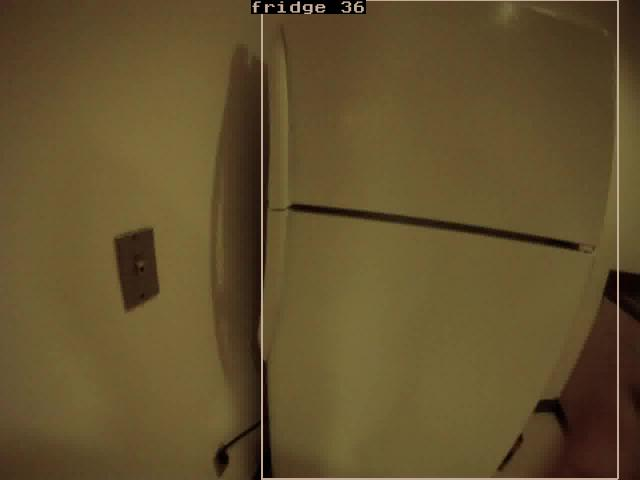
\includegraphics[width=2.0cm]{figures/fridge_passive.jpg}}}}
\subfigure[passive soap]{\bmvaHangBox{\fbox{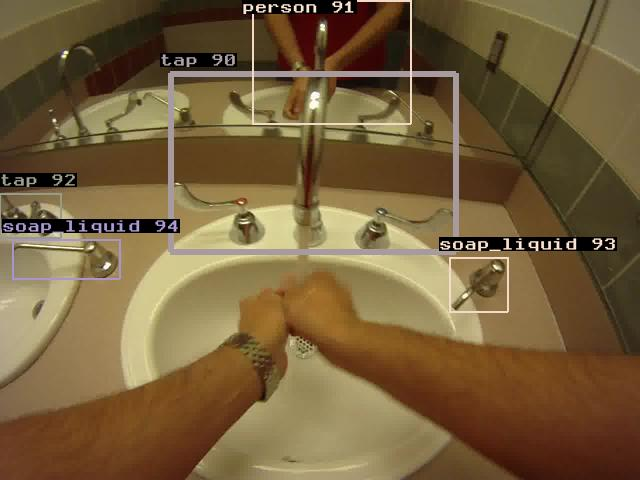
\includegraphics[width=2.0cm]{figures/soap_passive.jpg}}}}
\subfigure[passive mug]{\bmvaHangBox{\fbox{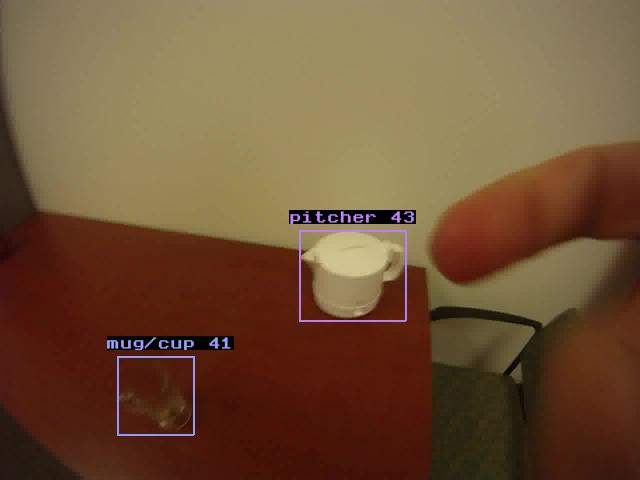
\includegraphics[width=2.0cm]{figures/mug_passive.jpg}}}}
\subfigure[passive micro]{\bmvaHangBox{\fbox{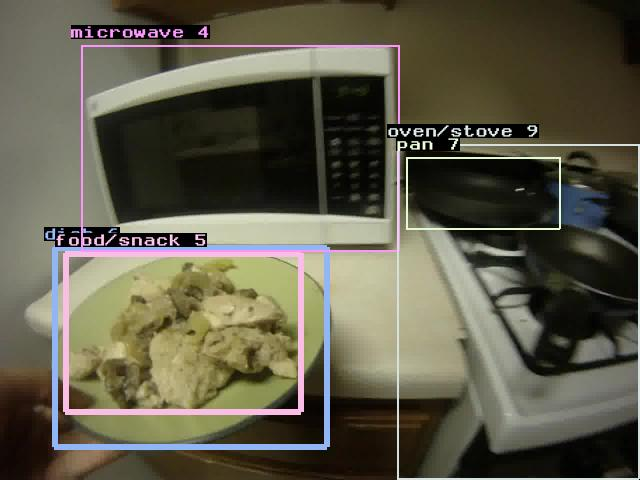
\includegraphics[width=2.0cm]{figures/micro_passive.jpg}}}}\\
\subfigure[active frig]{\bmvaHangBox{\fbox{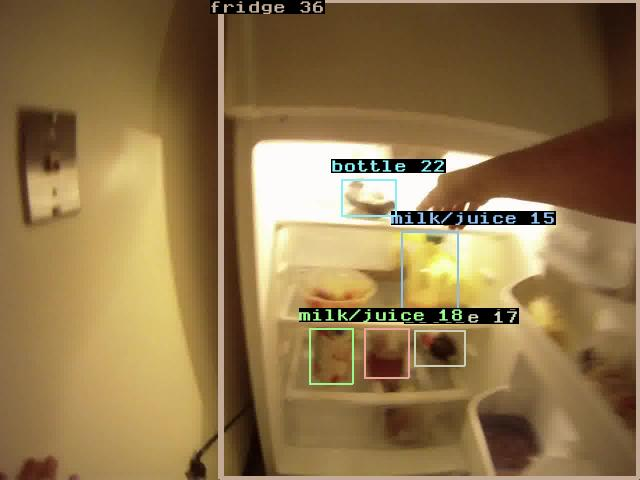
\includegraphics[width=2.0cm]{figures/fridge_active.jpg}}}}
\subfigure[active soap]{\bmvaHangBox{\fbox{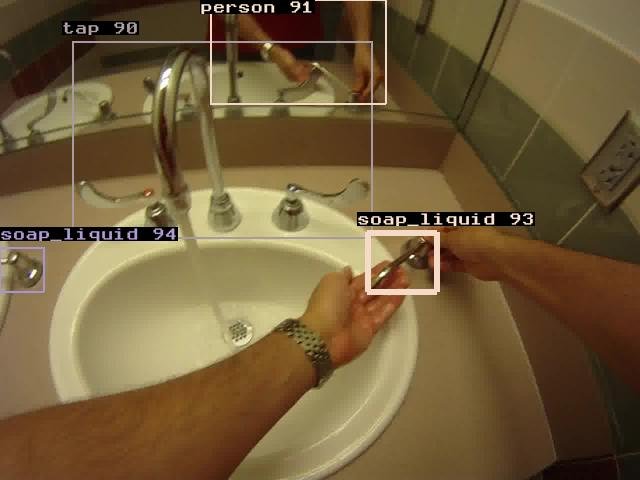
\includegraphics[width=2.0cm]{figures/soap_active.jpg}}}}
\subfigure[active mug]{\bmvaHangBox{\fbox{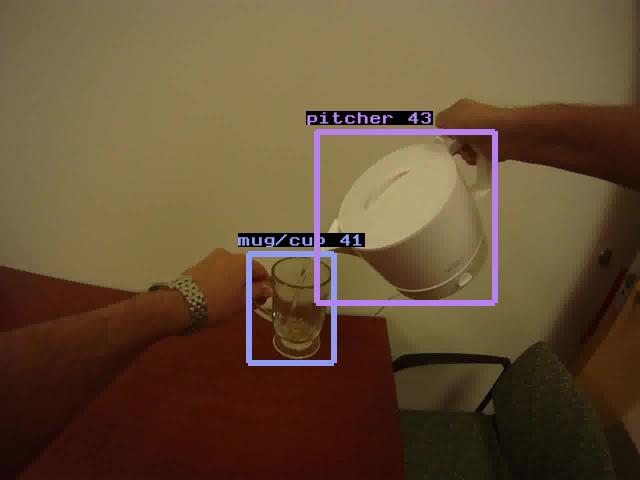
\includegraphics[width=2.0cm]{figures/mug_active.jpg}}}}
\subfigure[active micro]{\bmvaHangBox{\fbox{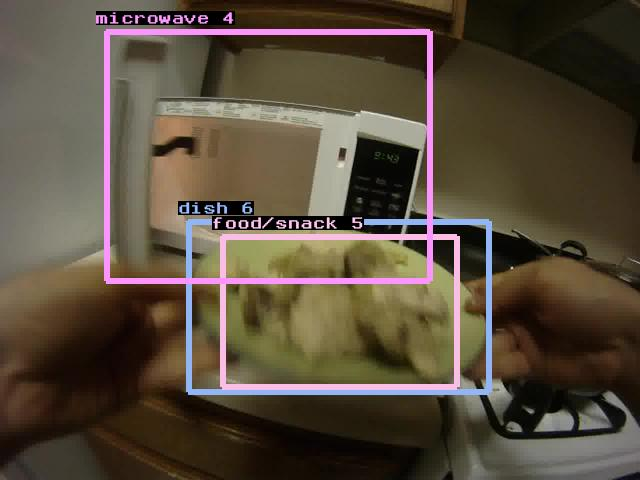
\includegraphics[width=2.0cm]{figures/micro_active.jpg}}}}
\end{tabular}
		   \caption{Example passive and active instances of four objects in ADL~\cite{Ramanan12}.}\vspace*{-0.2in}
\label{fig:active}
  \end{center}
 \end{figure}

 \vspace*{-0.05in}
\subsection{Detecting Active and Passive Objects}

Our goal is to robustly predict what type of activity is occurring in an egocentric video clip.  In contrast to traditional third-person video, egocentric actions are inherently defined by the objects the user is interacting with. Therefore, our representation is built on the pattern of objects that appear in space and time.  Specifically, the space-time pyramids we learn will count the frequency with which each object category appears in particular space-time regions.

Following~\cite{Ramanan12}, we make a distinction between active and passive instances of a given object category.  As noted in~\cite{Ramanan12}, objects' appearance can often change dramatically when the object is being interacted with.  For example, the refrigerator looks quite different when one passes by it closed, versus when one opens the door to grab some food.  Therefore, we train different deformable part model~\cite{DPM} detectors for active and passive versions of various objects of interest.\footnote{We use the public code and detection outputs provided by~\cite{Ramanan12}.}  Figure~\ref{fig:active} depicts example frames extracted from
the Activities of Daily Living (ADL)~\cite{Ramanan12} video sequences that show the visual differences between passive and
  active versions of four example objects.  In contrast to prior work, we exploit the active/passive object distinction to provide a helpful bias regarding where space-time partitions ought to be sampled, as we describe in the next section.
  
Once all object detectors have been applied to all frames in the training or test video, we have an $(x,y,t)$ coordinate for the bounding box center of each detected object.  Associated with each coordinate is its (predicted) object class (frig, microwave, etc.)


\subsection{Sampling Randomized Object-Centric Space-Time Pyramids}

Once we have the predicted object locations in all training videos, we are ready to construct space-time histogram pyramids.  A space-time pyramid will consist of multiple levels of bins, from coarse to fine.  For each bin, we record how many times each object class appears in its respective region of the video.  Then we concatenate these histograms over all pyramid levels to get a single descriptor for the video.  Thus, for a pyramid with $T$ total bins and a bank of $D$ total object detectors, the dimensionality of the entire descriptor will be $TD$.  Whereas past work uses a pyramid with uniformly placed bins~\cite{Choi08,Ramanan12}, we propose to generate randomized pyramids and then learn their most discriminative combination.

First we describe how to generate the randomized space-time pyramids (RSTP) \emph{without} the object-centric bias.  We consider each dimension $(x,y,t)$ in turn in a round-robin fashion to generate a cut (i.e., place a bin boundary).  Each cut is axis-aligned, meaning we use random shifts, but no random rotations.  We normalize all dimensions of an input video to length 1.  Then we sample a number uniformly at random in $[0,1]$, and use it to place the randomized cut in the current dimension.  Note that as we work our way recursively down the resulting tree, each subsequent cut is appropriately constrained by the span of its parent bin.  Level 0 of the pyramid is the entire video clip volume; level $i$ consists of all $8^i$ bins of depth $i$.

While boosting gives an automated way to select informative pyramids, its training time depends linearly on the number of candidates we include in the pool.  With so many possible randomized pyramids, the search space is extremely large.  Thus, intuitively, we can expect to pay a very high training cost to evaluate sufficiently many randomized pyramids to get good results.  

To avoid an excessive search, we focus the candidate pool in a way that is meaningful for egocentric data.  Rather than sample cuts uniformly at random, our idea is to sample the cuts according to the distribution of active objects as they appear in the training videos.  We refer to these as \emph{object-centric cuts} (OCC).  Specifically, we construct the empirical distribution of all active object occurrences, per dimension.  Then, when selecting each randomized cut, we sample its position according that distribution.  In this way we get pyramids that emphasize video regions likely to characterize the interactions between the camera wearer and objects.  For each pyramid, after generating one OCC per dimension, we generate all subsequent child cuts using a uniform distribution.  We found this was more effective than using OCC's at all levels, likely because we risk overfitting once bins are quite small in volume.  Note that while the OCC's are biased by active objects only, we still count both active and passive objects in the resulting histograms.



\begin{figure}
  \begin{center}
\begin{tabular}{ccc}
\bmvaHangBox{\fbox{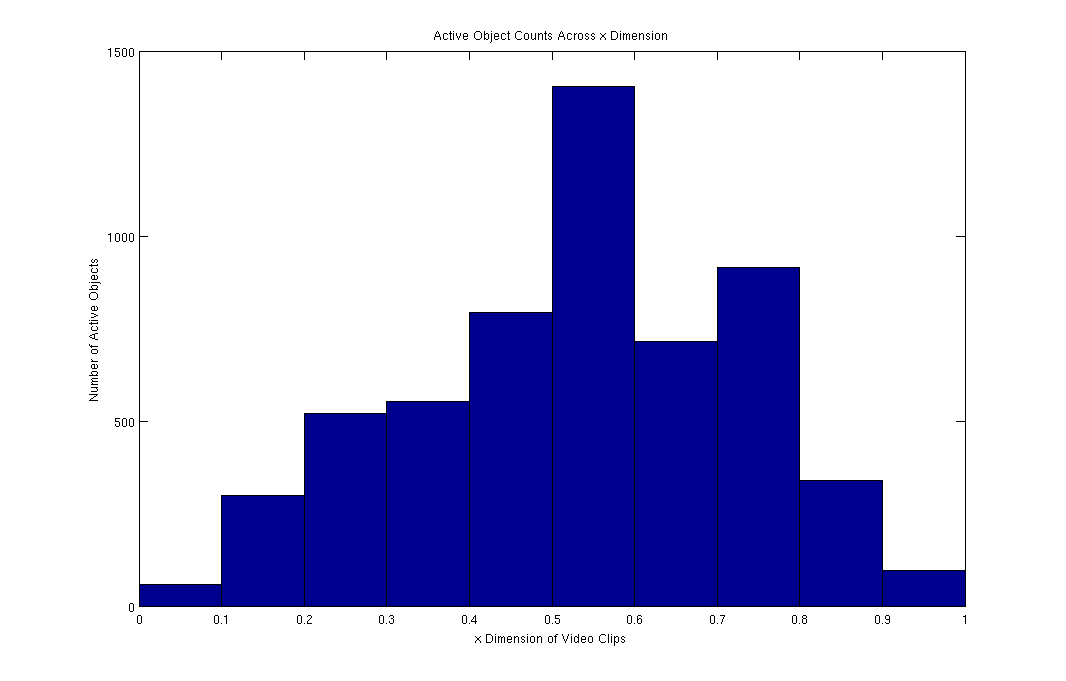
\includegraphics[width=3.5cm]{figures/active_obj_distr_x.png}}}&
\bmvaHangBox{\fbox{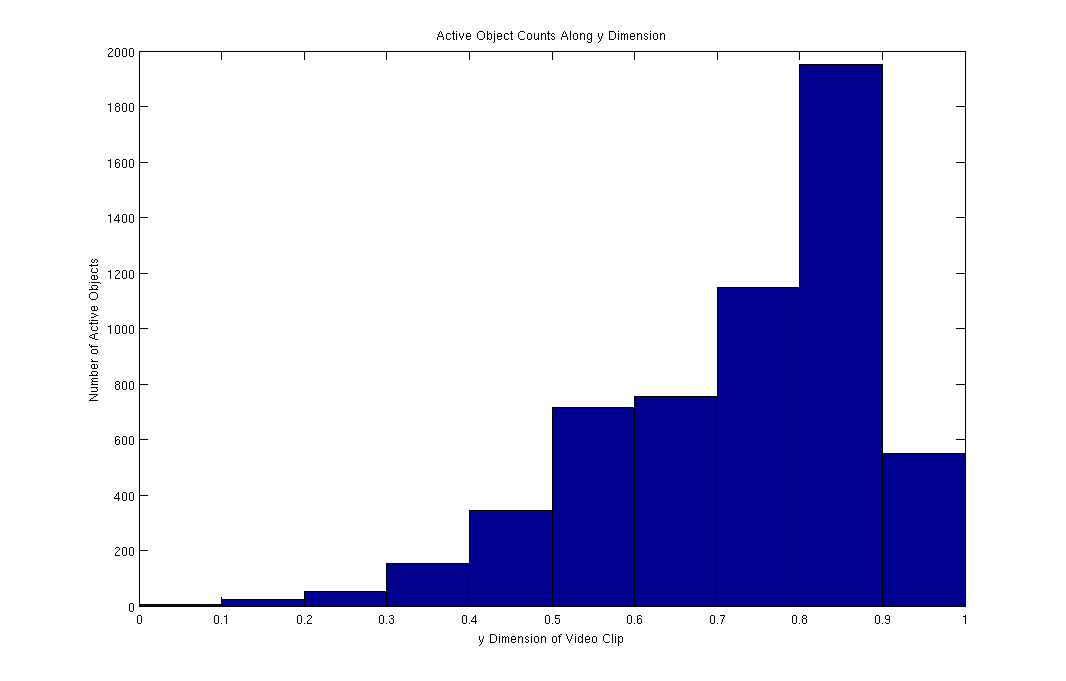
\includegraphics[width=3.5cm]{figures/active_obj_distr_y.png}}}
\bmvaHangBox{\fbox{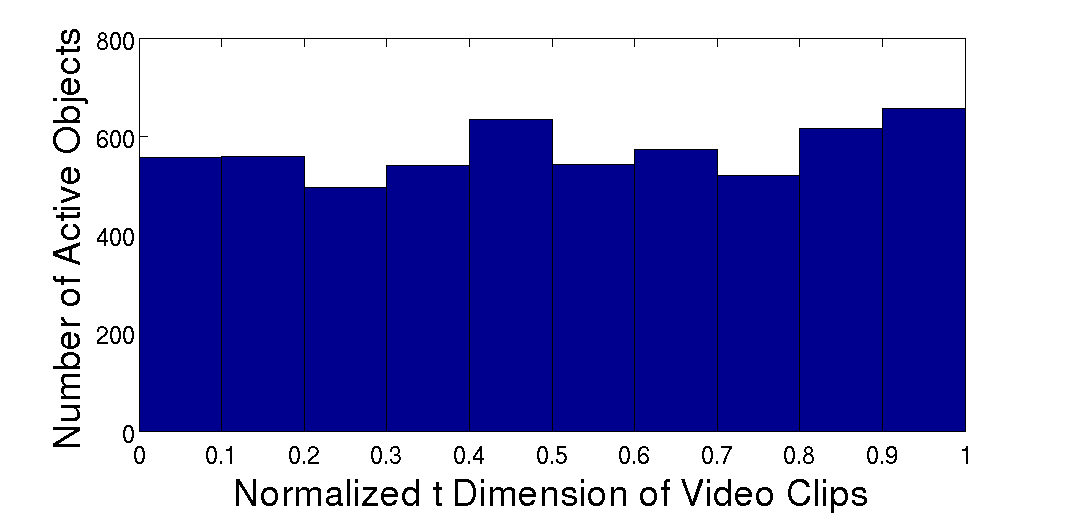
\includegraphics[width=3.5cm]{figures/active_obj_distr_t.png}}}
\end{tabular}
		   \caption{Histograms of detected active objects across $x$, $y$, and $t$ in the training data.}
\label{fig:histograms}
  \end{center}

\end{figure}


Figure~\ref{fig:histograms} shows the active object distributions for the ADL dataset we use to validate our approach.  We see that active objects tend to appear in the lower center field of view.  This conforms to our expectations, because active objects are close to the hands, which appear in the bottom portion of most frames from the chest mounted camera.  Furthermore, there is a slight bias favoring the right side of the field of view, likely because many camera wearers are right-handed.  Finally, we also observe that the distribution of active objects
  across the temporal dimension is nearly uniform; this reflects that we use object occurrences across all action types.  %%An alternative would be to generate action class-specific partitions.  Doing so might allow even more precise partitions, though will be more expensive for training.
  
  
%
%	\begin{figure}[t]
%		\begin{center}
%			%\fbox{\rule{0pt}{2in} \rule{0.9\linewidth}{0pt}}
%%			  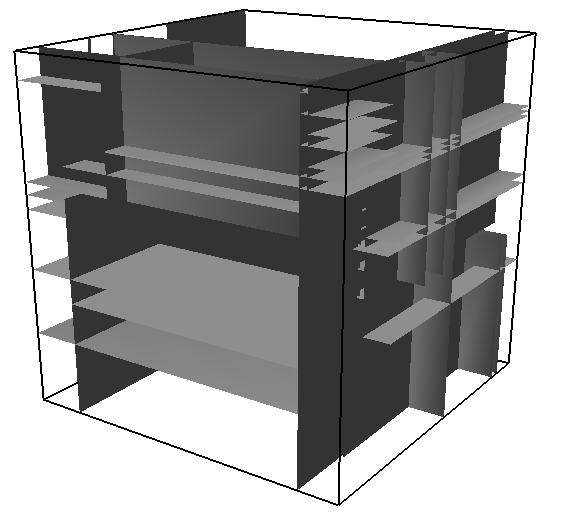
\includegraphics[width=6.0cm]{figures/lvl3-3.png}
% 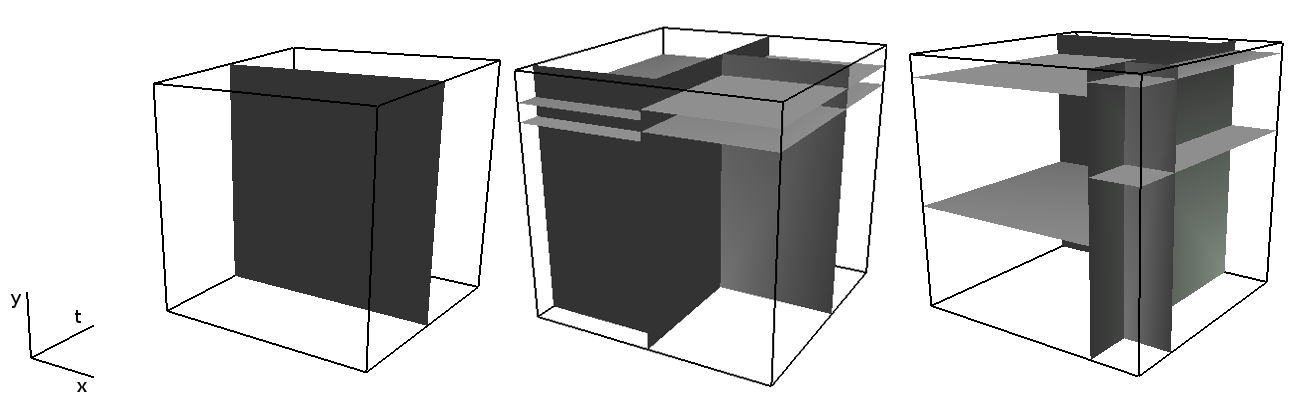
\includegraphics[width=6.0cm]{figures/allpyramids_axes.png}
%		\end{center}
%    \caption{temporal, unbiased, biased.  UPDATE An example 3-level object-centric partitioning scheme. Visible cuts along
%    the $y$ dimension correspond to locations known to frequently contain
%  active objects.}\label{fig:3types}
%	\end{figure}

Figure~\ref{fig:2dpartitions} shows some example frames with randomized shifts sampled using our object-centric strategy (a) or the simpler uniform strategy (b).  The object detections shown are from the ADL repository~\cite{Ramanan12}.  We see how OCC's successfully focus the histograms on regions in space-time where human-object interactions occur.  As a result, they may offer more discriminative cues that will be useful to the boosted classifier.

%
%  Figure 3 depicts an example 3-level object-centric partition scheme.
%  The salient feature to note is that visible splits along the $y$
%  dimension correspond to the observed distribution of active objects along
%  the $y$ dimension of the training data.
%




\begin{figure}[t]
  \begin{center}
  \begin{tabular}{c}
  \subfigure[Object-centric cuts]{
\begin{tabular}{ccccc}
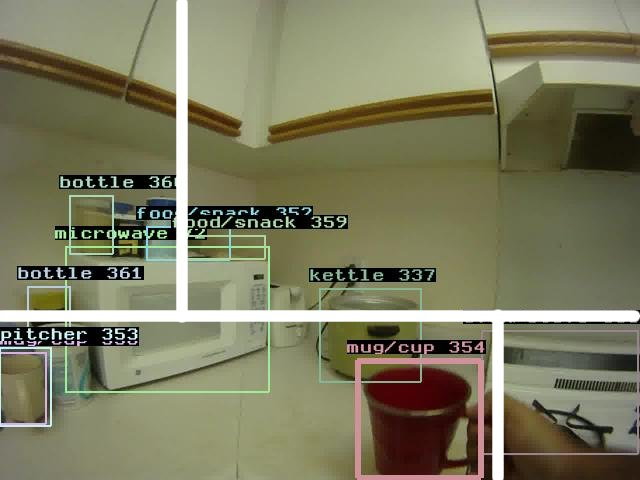
\includegraphics[width=2.2cm]{figures/ex1_biased.jpg}
%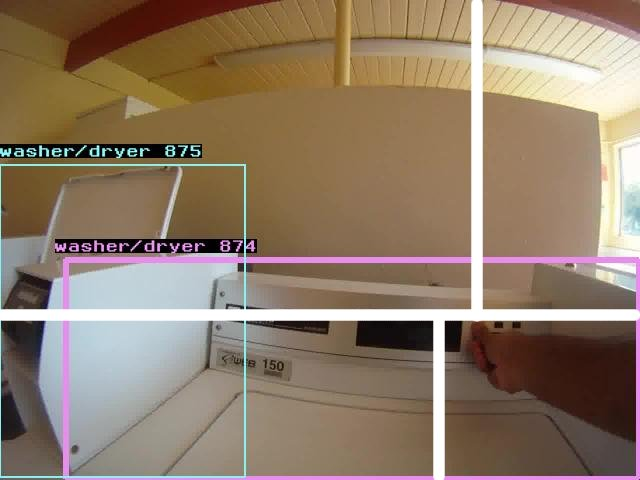
\includegraphics[width=2.2cm]{figures/ex2_biased.jpg}
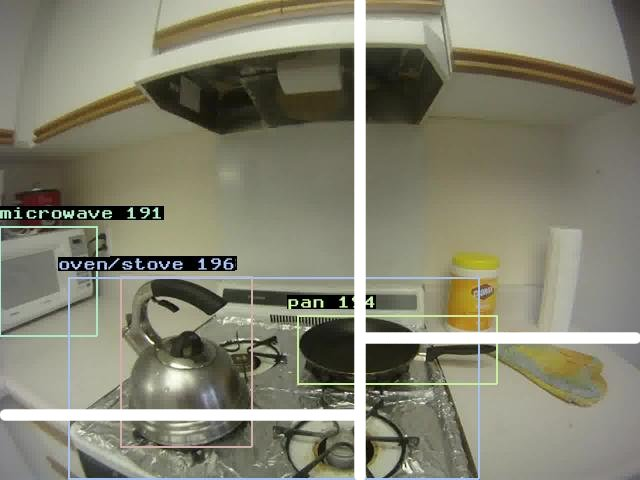
\includegraphics[width=2.2cm]{figures/ex3_biased.jpg}
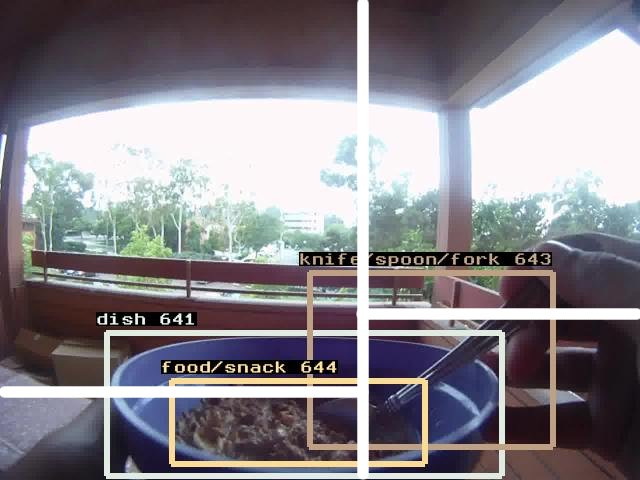
\includegraphics[width=2.2cm]{figures/ex4_biased.jpg}
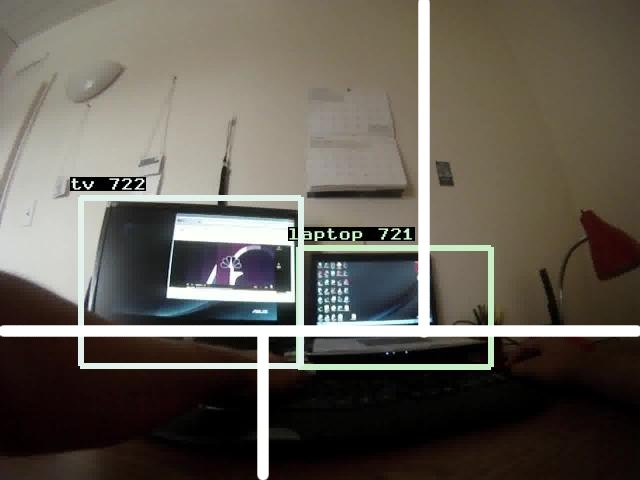
\includegraphics[width=2.2cm]{figures/ex5_biased.jpg}
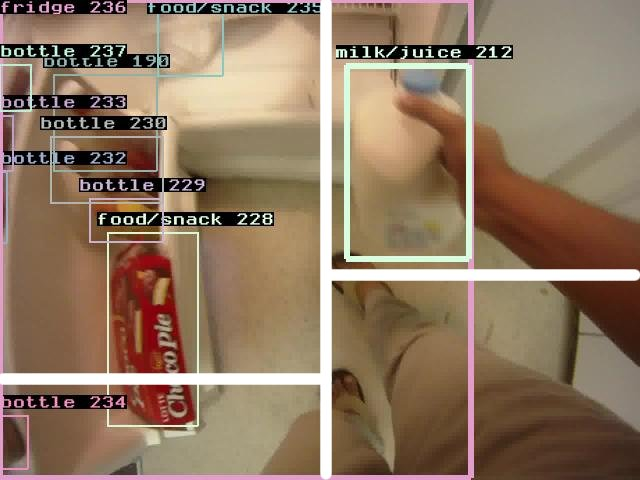
\includegraphics[width=2.2cm]{figures/ex6_biased.jpg}
\end{tabular}}\\
 \subfigure[Uniformly random shifts]{
\begin{tabular}{ccccc}
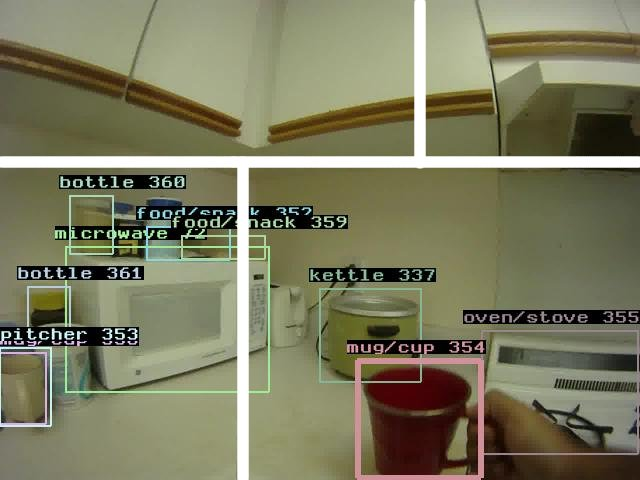
\includegraphics[width=2.2cm]{figures/ex1_unbiased.jpg}
%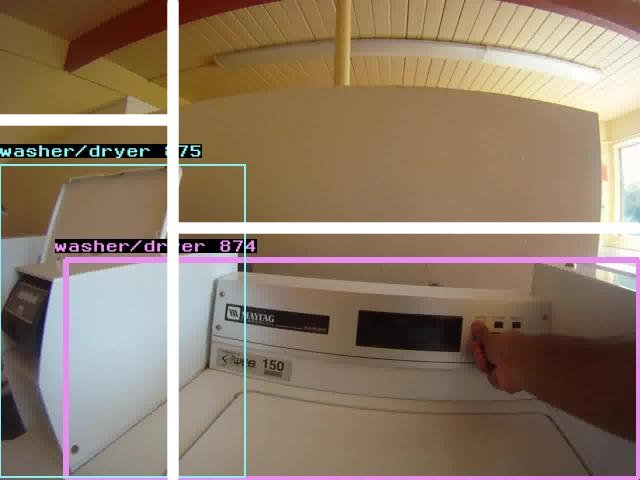
\includegraphics[width=2.2cm]{figures/ex2_unbiased.jpg}
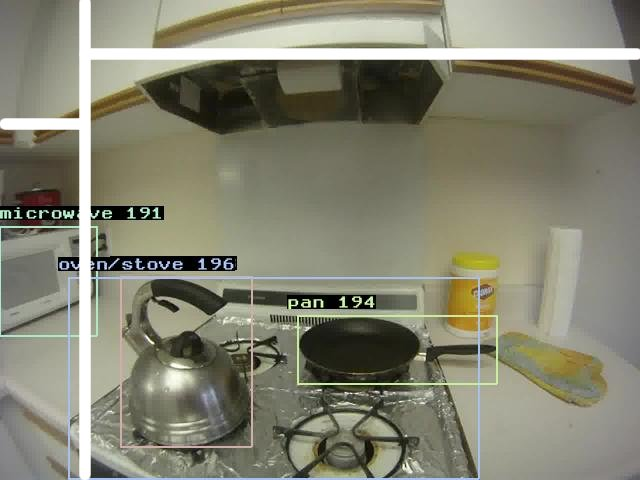
\includegraphics[width=2.2cm]{figures/ex3_unbiased.jpg}
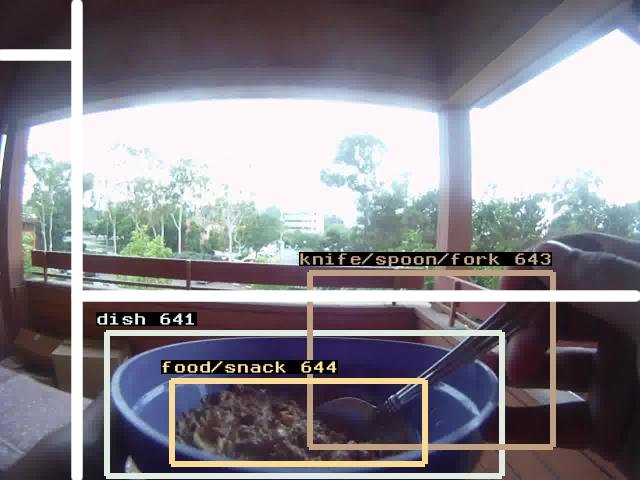
\includegraphics[width=2.2cm]{figures/ex4_unbiased.jpg}
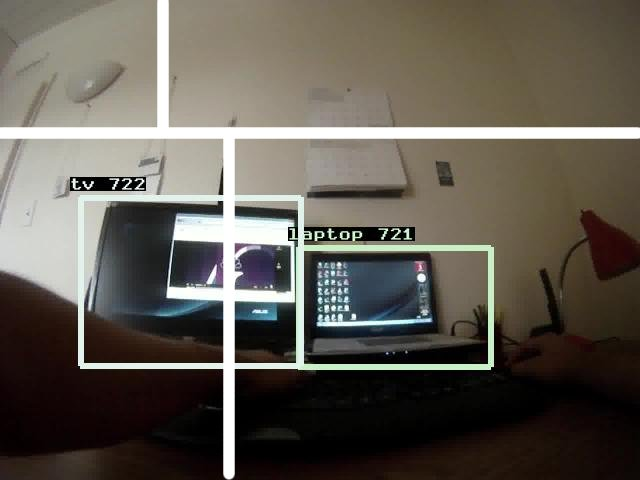
\includegraphics[width=2.2cm]{figures/ex5_unbiased.jpg}
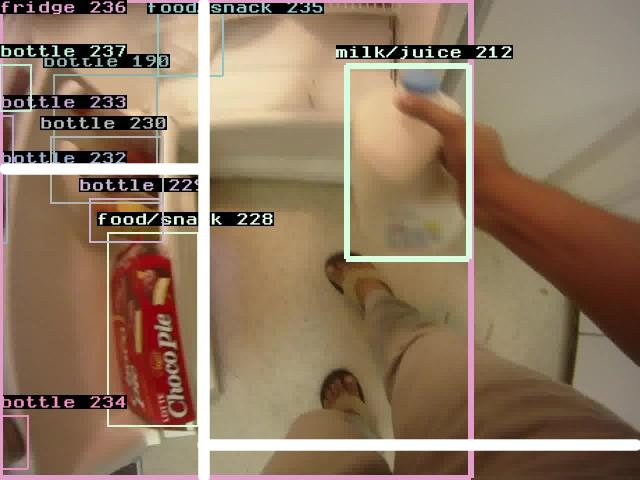
\includegraphics[width=2.2cm]{figures/ex6_unbiased.jpg}
\end{tabular}}
\end{tabular}
%\bmvaHangBox{\fbox{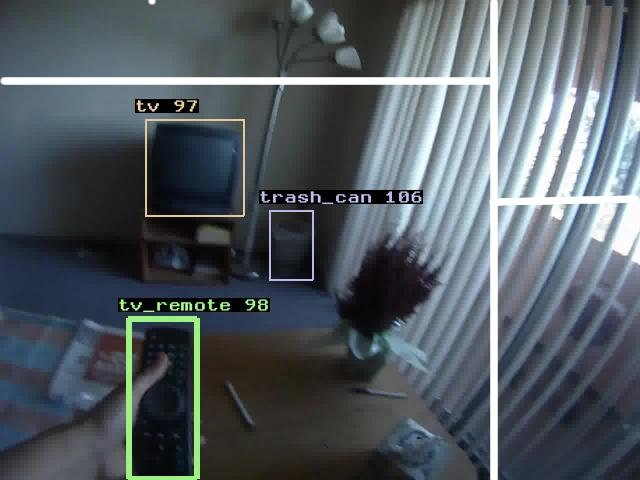
\includegraphics[width=5.9cm]{figures/unbiased_prt.jpg}}}&
%\bmvaHangBox{\fbox{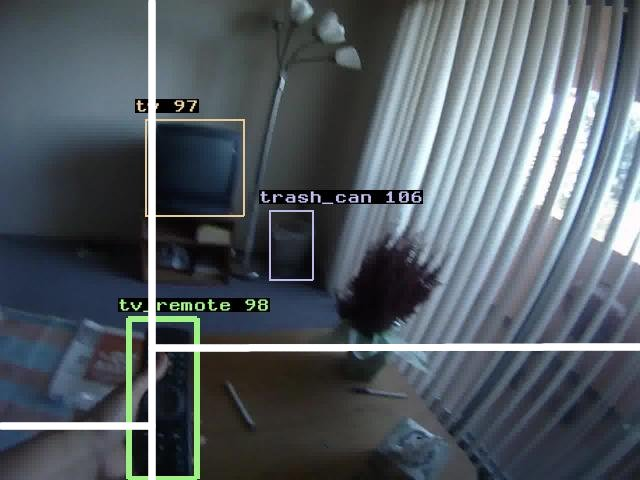
\includegraphics[width=5.9cm]{figures/biased_prt.jpg}}}\\
		   \caption{Example partitions using either object-centric (a) or uniformly sampled randomized cuts (b).  Note that for display purposes we show cuts on example 2D frames, but all cuts are 3D in space-time.  Using the proposed object-centric cuts, we better focus histograms surrounding the human-object interactions.}
\label{fig:2dpartitions}
  \end{center}
\end{figure}



\subsection{Boosting Discriminative Space-Time Pyramids}



\begin{figure}[t]
  \begin{center}
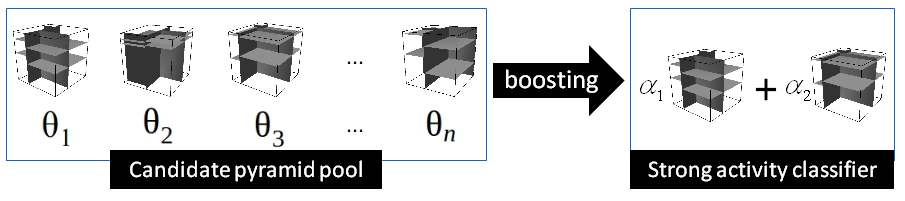
\includegraphics[width=9cm]{figures/concept-alg.png}
		   \caption{We take a pool of randomized space-time pyramids with object-centric cuts, and use boosting to select those that are most discriminative for egocentric activity recognition.}
\label{fig:concept-alg}
  \end{center}
\end{figure}


Finally, having constructed our object-centric pool of randomized pyramids, we are ready to apply boosting to select those that are most discriminative for the given activity recognition task (see Figure~\ref{fig:concept-alg}).  Boosting is a general learning algorithm in which one can combine a series of ``weak'' classifiers (better than chance) to form a single ``strong'' classifier.  In each round of boosting, the training examples are reweighted to emphasize training errors on those examples that were misclassified by weak classifiers selected in previous rounds. Here, our weak classifiers are non-linear (polynomial kernel) SVMs trained using one RSTP with OCC's.  We essentially use boosting to both select useful features (pyramids) and build the composite strong classifier.

For our implementation, we use the Stagewise Additive Modeling using a Multi-class Exponential loss function (SAMME) boosting approach of~\cite{Zhu06}, which naturally extends the original AdaBoost algorithm to the multi-class case without reducing it to multiple two-class problems.  We chose it due to its advantage of avoiding training individual classifiers for many one-vs.-rest (or one-vs.-one) problems and due to its ease of implementation.

SAMME boosting works as follows in our setting.  We take as input a collection of $N$ labeled training videos, where $(V_i, c_i)$ denotes a video clip and its associated ground-truth  activity label (drinking water, washing dishes, etc.).  We generate a pool of $M$ candidate RSTP's  $\{\theta_1, \theta_2, ..., \theta_M\}$, as described above.  For each RSTP $\theta$, we compute the corresponding histogram for each training example, using an object's bounding box center position $(x,y,t)$ to increment the appropriate bins.  We concatenate the histograms from all levels to create a single feature vector for each $V_i$ and each $\theta$.  Then we initialize a weight $w_i$ for each training example $V_i$ that is inversely proportional to the number of points with the same label as $V_i$. Giving larger weights to training examples of infrequently occurring actions helps to mitigate bias from imbalanced training data.

Next we train a separate weak multi-class SVM classifier (using the one-vs.one protocol in LIBSVM \cite{Chang11})
	 on the feature vectors resulting from representing the training
	data using each candidate partition pattern. 
 During each round of boosting we select the
	candidate partition $\theta_j$ that has the minimum  weighted training error.
  SAMME computes a weight for $\theta_j$ based on how many training
  examples were misclassified using $f_{\theta_j}$, the SVM classifier
  that was trained using the representation of the training data under
  $\theta_j$.
  At the end of each boosting iteration, we update the weights for each
  training example. Training examples that were previously misclassified are
  assigned higher weights to encourage correct classification in future
  boosting rounds.  Finally, we generate the
	final strong classifier $F$, which maximizes a weighted
  sum of correct classifications produced by each weak classifier.   Algorithm 1 summarizes these steps.
  
  Given a novel input video, we run the object detectors, then extract only those RSTP histograms that were selected by boosting, and apply $F$ to predict its activity label.
  
  %
%	\noindent\textbf{Algorithm 1:} Training via Multi-Class Boosting \\
%	\textbf{INPUT:}
%	\begin{itemize}
%		\item $N$ labeled training videos $\Phi = \{(V_i, c_i)\}_{i=1}^N$
%		\item A pool of $M$ partition patterns $\Theta = \{\theta\}$
%	\end{itemize}
%	\textbf{OUTPUT:}
%	\begin{itemize}
%		\item A strong video classifier $F$. For an unlabeled video $V$,
%			$c=F(V)$ is the predicted label for $V$.
%	\end{itemize}
%			\begin{enumerate}
%
%				\item For each $\theta \in \Theta$:
%					\begin{itemize}
%            \item Compute the representations of each $V_i \in \Phi$ using $\theta$
%						and train a multi-class classifier (SVM) $f_\theta$ on the
%            resulting feature vectors.
%					\end{itemize}
%
%				\item Initialize:
%					\begin{itemize}
%						\item A weight $w_i = \frac{1}{C N_{c_i}}$ for each video clip,
%							where $N_{c_i}$ is the number of videos with label $c_i$,
%              and $C$ is the number of distinct labels in the training data.
%						\item Current boosting round $j=0$.
%						%\item Current accuracy $\sigma_j = 0$.
%					\end{itemize}
%
%				\item For each round of boosting:
%					\begin{itemize}
%						\item Increment $j$.
%						\item Re-normalize the weight vector:
%              \begin{center}
%              $\forall i, w_i = \frac{w_i}{\Sigma_i^N w_i}$.
%              \end{center}
%					  \item For each pattern $\theta$,
%              compute its weighted classification error:
%              \begin{center}
%              $e_\theta = w \cdot \mbox{\textbf{I}}(f_\theta(V) \neq c)$
%              \end{center}
%						\item Choose the pattern $\theta_j$ with minimum weighted
%              classification error $e_j$.
%						\item Compute the weight for $\theta_j$:
%              \begin{center}
%              $\alpha_j = \mbox{log} \frac{1 - e_j}{e_j} + \mbox{log}(C-1)$
%              \end{center}
%						\item Update the weight vector:
%              \begin{center}
%							$w_i = w_i \cdot \mbox{exp}(\alpha_j \cdot
%							\mbox{\textbf{I}}(f_{\theta_j}(V_i) \neq c_i))$.
%              \end{center}
%						\item Generate the current strong classifier:
%              \begin{center}
%							$F(V) = \mbox{argmax}_c \Sigma_{m=1}^j \alpha_m \cdot
%							\mbox{\textbf{I}}(f_{\theta_m}(V) = c)$
%              \end{center}
%					\end{itemize}
%
%			\end{enumerate}
%	

  \footnotesize
  \hspace*{-0.19in}\line(1,0){365}\\
  \noindent\textbf{Algorithm 1:} Training a space-time pyramid classifier with boosting \\
  \line(1,0){365}\\
  \textbf{\scriptsize INPUT:}
  \begin{itemize}
    \item $N$ labeled training videos $\Phi = \{(V_i, c_i)\}_{i=1}^N$
    \item A pool of $M$ partition patterns $\Theta = \{\theta\}$
  \end{itemize}
  \textbf{\scriptsize OUTPUT:}
  \begin{itemize}
    \item A strong video classifier $F$. For an unlabeled video $V$,
      $c=F(V)$ is the predicted label for $V$.
  \end{itemize}
      \begin{enumerate}
        \item For each pattern $\theta \in \Theta$:
          \begin{itemize}
            \item Represent each $V_i \in \Phi$ using $\theta$
            and train an SVM classifier $f_\theta$ on the
            resulting feature vectors.
          \end{itemize}

        \item Initialize:
          \begin{itemize}
            \item A weight vector $w$ with $w_i = \frac{1}{C N_{c_i}}$ for each video
              where
              $N_{c_i}$ is the number of videos with label $c_i$, and
              $C$ is the number of distinct action labels.
            \item Current boosting round $j=0$.
          \end{itemize}

        \item For each round of boosting:
          \begin{itemize}
            \item Increment $j$ and re-normalize the weight vector $w$.
            \item For each pattern $\theta$,
              compute its weighted classification error:
              $\;\;\;\;e_\theta = w \cdot \mbox{\textbf{I}}(f_\theta(V) \neq c)$
            \item Choose the pattern $\theta_j$ with minimum weighted
              classification error $e_j$.
            \item Compute the weight for $\theta_j$ as:
              $\;\;\;\;\alpha_j = \mbox{log} \frac{1 - e_j}{e_j} + \mbox{log}(C-1)$
            \item Update the weight vector $w$:
              $\;\;\;\;\forall i: w_i = w_i \cdot \mbox{exp}(\alpha_j \cdot
              \mbox{\textbf{I}}(f_{\theta_j}(V_i) \neq c_i))$.
            \item Generate the current strong classifier as:
              $\;\;\;\;F(V) = \mbox{argmax}_c \Sigma_{m=1}^j \alpha_m \cdot
              \mbox{\textbf{I}}(f_{\theta_m}(V) = c)$
          \end{itemize}
      \end{enumerate}
  \line(1,0){365}\\
  \normalsize

  
  














%
%
%  \subsection{Complexity and Runtime}
%  The asymptotic complexity of training with $N$ training examples
%  and a pool of $M$ candidate partition schemes with $l$ levels using our
%  method is
%  \begin{center}
%  $O(N\cdot M \cdot 8^l \cdot t_{train} + b \cdot (N + M \cdot t_{test}))$
%  \end{center}
%  where $b$ denotes the number of boosting rounds, and $t_{train}$ and
%  $t_{test}$ denote the time to train and test a single SVM classifier on
%  $N$ feature vectors, respectively. Fortunately, $l$ remains small (never
%  exceeds 4 in our experiments). In order to predict the label for a single
%  test video clip $v$, we first need to compute representations of $v$ using
%  each partition scheme that was selected during boosting, then find the
%  class $c$ which maximizes a weighted sum of matching classifications using
%  each weak classifier selected during boosting.
%  Thus, the overall
%  asymptotic complexity of predicting the
%  label for a single video clip is
%  \begin{center}
%  $O(b \cdot 8^l + C \cdot b \cdot t)$
%  \end{center}
%  where $b$ is the number of boosting rounds, $C$ is the number of possible
%  activity labels, and $t$ is the time to predict the label of a test
%  example using a weak SVM classifier.
%
